\documentclass{article}

\usepackage[hyphens]{url} 


\usepackage[utf8]{inputenc}

\usepackage{pdfpages}
\usepackage{lastpage}
\usepackage{fancyhdr}
\usepackage{ngerman}
\usepackage{listings}
\usepackage{hyperref}
\usepackage{tabularx}
\usepackage{floatrow}
\usepackage[tableposition=top]{caption}
\floatsetup[table]{capposition=top}

\usepackage{amsmath, amssymb}

\usepackage[utf8]{inputenc}

\usepackage{xifthen}
\usepackage[numbib]{tocbibind}

\newcommand\twodigits[1]{%
   \ifnum#1<10 0#1\else #1\fi
}



\lhead{Halbleiterdiode}
\rhead{27. November 2020\\T. Maier, J. Winkler}
%\cfoot{\twodigits{\thepage}~/ \pageref{LastPage}}
\cfoot{{\thepage}~/ \pageref{LastPage}}

\newcommand{\W}{\text{W}}
\newcommand{\V}{\text{V}}
\newcommand{\A}{\text{A}}

\newcommand{\UR}{$U_R$ }
\newcommand{\UIR}{$U_\text{IR}$ }

\newcommand{\mini}{\operatorname{min}}


\begin{document}

\parindent0cm

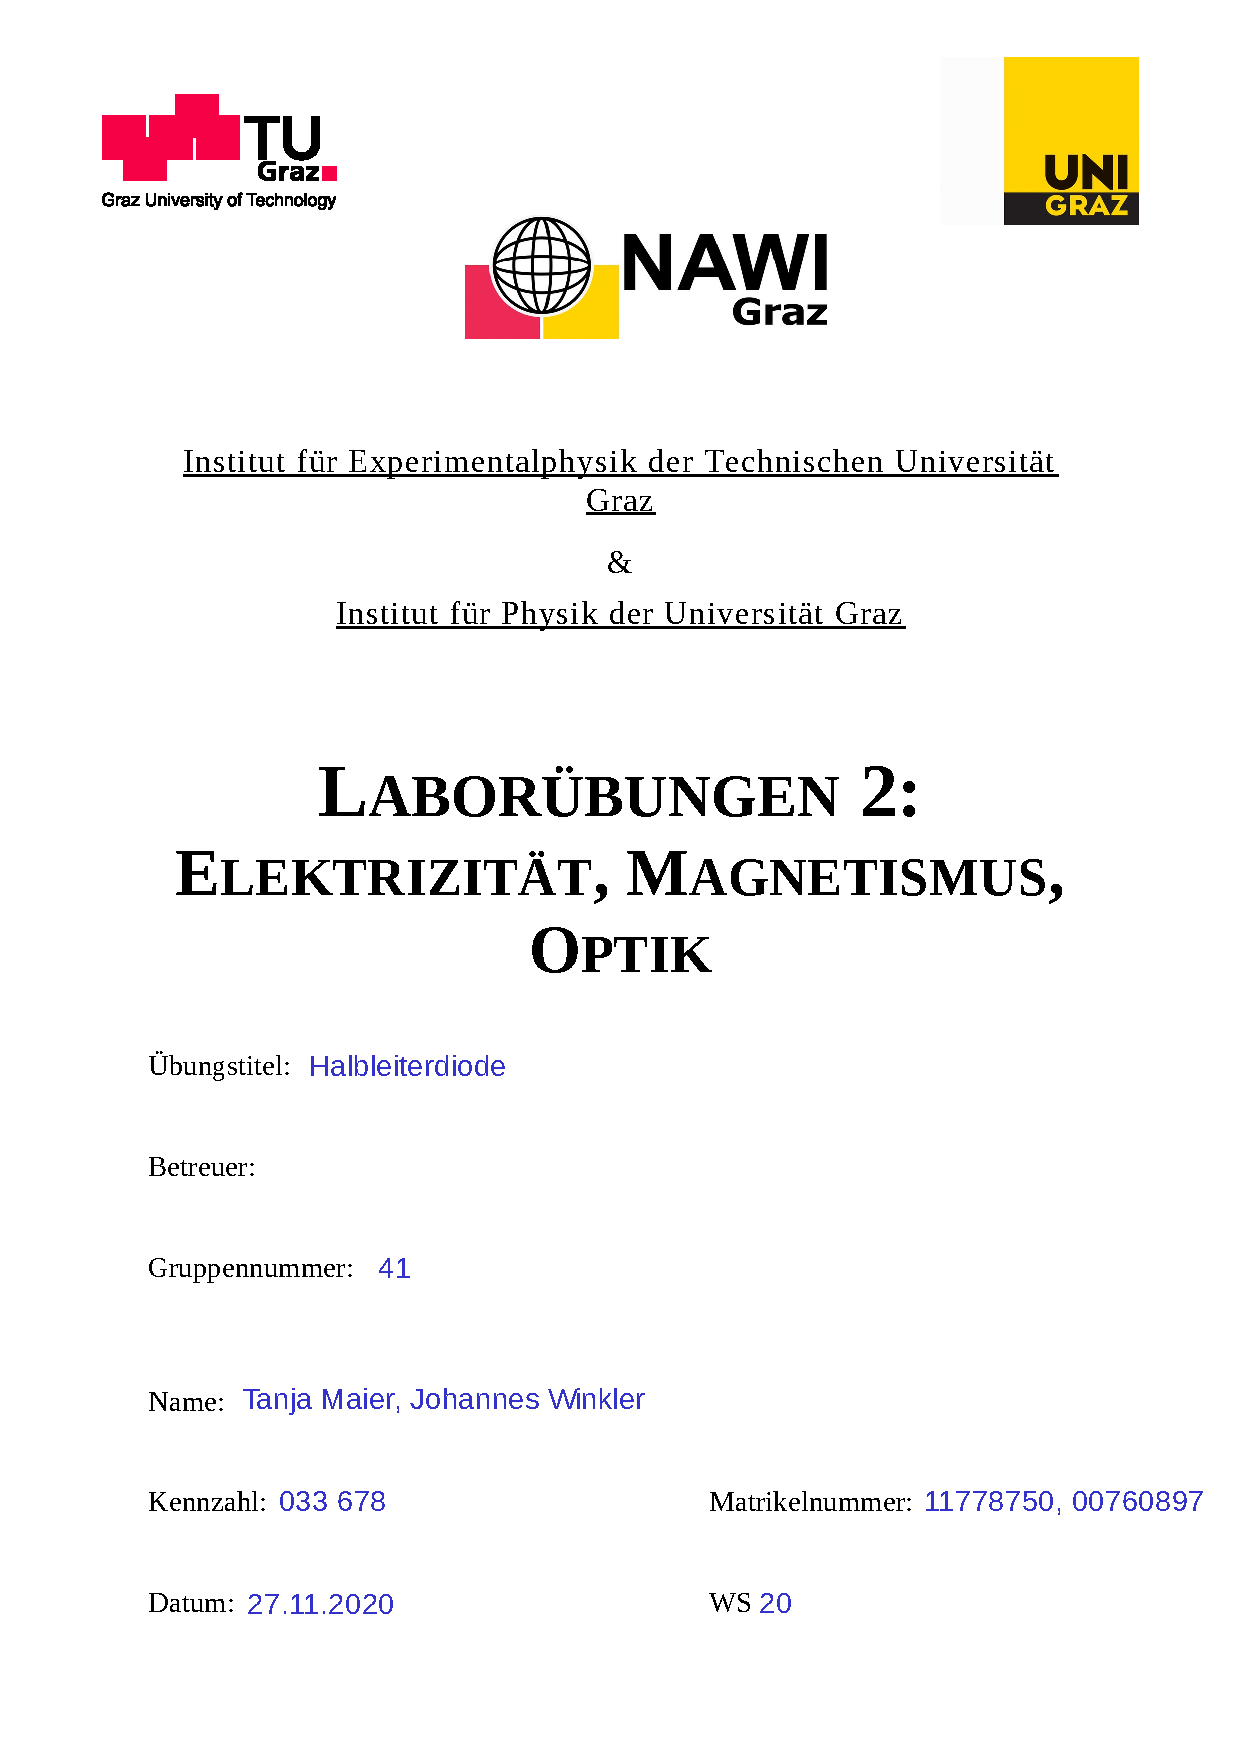
\includepdf{Deckblatt.pdf}


\pagestyle{fancy}

\tableofcontents
\newpage
\section{Aufgabenstellung}



\begin{enumerate}
\item Messtechnische Ermittlung der Strom-Spannungscharakteristik einer Gleichrichterdiode in Durchlassrichtung und in Sperrrichtung.
\item Automatisierte Aufnahme der Strom-Spannungscharakteristik einer Zenerdiode in Durchlassrichtung und Sperrrichtung.
\item Messtechnische Untersuchung von Spannungs- und Stromverläufen in einer Einweg- bzw. Gleichrichterschaltung mit unterschiedlichen Glättungskondensatoren und Belastungswiderständen.
\end{enumerate}



\section{Voraussetzungen und Grundlagen}

\subsection{Halbleiter und Leitfähigkeit}

Als Halbleiter bezeichnet man einen kristallinen Feststoff, der aufgrund von seiner elektrischen Leitfähigkeit sowohl als Leiter als auch als Nichtleiter gesehen werden kann. Die Leitfähigkeit ist dabei stark temperaturabhängig, im Bereich des absoluten Nullpunktes sind Halbleiter praktisch nicht leitfähig (da so gut wie keine frei beweglichen Elektronen vorhanden sind) und verhalten sich wie Isolatoren. Nicht elektrisch leitfähige Halbleiter werden auch als ideale Halbleiterkristalle bezeichnet und besitzen trotz der fehlenden Ladungsträger eine gewisse Oberflächenleitfähigkeit, die durch das Fehlen der Partneratome an den Grenzflächen und den damit verbundenen „Defektelektronen“ begründet werden kann. Solche Effekte treten auch im Inneren des Kristalles auf und tragen zur Eigenleitfähigkeit des Halbleiters bei.
Die elektrische Leitfähigkeit von Halbleitern nimmt mit steigender Temperatur zu, sie werden deshalb auch als Heißleiter bezeichnet. (vgl. \cite{moodle}, \cite{halbleiter})


\subsection{Bänder und Halbleiter}

Das Bändermodell ist ein quantenmechanisches Modell, mit dem elektronische Energiezustände in einem Kristall und somit die Leitfähigkeit von Leiter, Halbleitern und Isolatoren beschrieben werden kann. Ausgegangen wird davon, dass sich die Atomrümpfe in einem festen Gitter, also an fixen Positionen im Kristall befinden. Der Bereich der Ladungsträger wird dann in Valenzband, Bandlücke und Leitungsband aufgeteilt. Die Elektronen befinden sich zunächst im Valenzband, im Grundzustand ist das Leitungsband nicht besetzt. Die jeweilige Größe der Bandlücke entscheidet über die elektrische Leitfähigkeit. (vgl. \cite{moodle}, \cite{halbleiter})


\begin{figure}[H]
\caption{Bändermodell}
\label{fig:baender}
{\centering
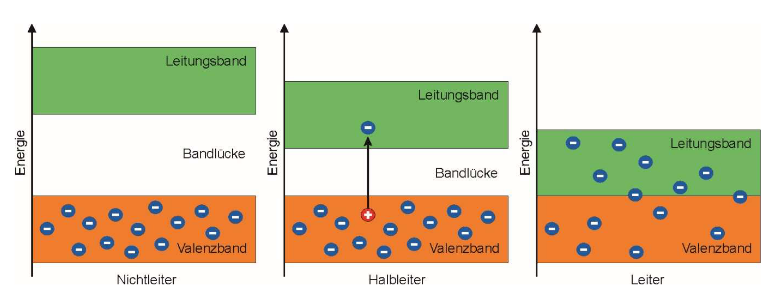
\includegraphics[scale=1.7]{baender.png}
~
}
\end{figure}


Bei elektrischen Leitern ist das Valenzband entweder nicht vollständig besetzt oder Valenzband und Leitungsband überlappen sich – die Bandlücke ist also nicht vorhanden. Dies ermöglicht den Elektronen sich frei über das Valenzband und Leitungsband zu bewegen. Elektrische Leiter sind beispielsweise Metalle wie Kupfer oder Aluminium. (vgl. \cite{moodle}, \cite{cosmos}, \cite{greenlane})

~

Bei Halbleitern ist die Bandlücke gerade so groß, dass zumindest ein Teil der Elektronen bereits bei geringer Anregung (z.B. Raumtemperatur) vom Valenzband in das Leitungsband gelangen. Jedes Elektron, das so in das Leitungsband gelangt hinterlässt dabei eine Lücke im Valenzband, die durch ein weiteres Elektron aus „dem Inneren“ wieder aufgefüllt werden muss. So entsteht der Eindruck als würde die Lücke immer weiterwandern. Wichtig zu beachten ist, dass es dabei immer gleich viele positive Ladungen (Lücken) und negative Ladungen im Valenzband gibt – der Halbleiterkristall ist also insgesamt elektrisch neutral. Eines der wichtigsten Halbleitermetalle ist Silizium. (vgl. \cite{moodle}, \cite{lernhelfer})

~

Bei Isolatoren ist die Bandlücke so groß, dass kein Elektron vom Valenzband in das Leitungsband gelangt. Die Elektronen sind also im Valenzband „eingesperrt“ und könnten, wenn überhaupt nur mit großem Energieaufwand stark genug angeregt werden, um in das Leitungsband zu gelangen. Als Isolatoren geeignete Materialien sind zum Beispiel Gummi oder Glas. (vgl. \cite{moodle}, \cite{cosmos}, \cite{greenlane})


\subsection{Dotierung von Halbleitern}


Das Dotieren beschreibt das Einbringen von Fremdatomen in den Halbleiter, um so gezielt seine Leitfähigkeit zu verändern. Man unterscheidet dabei zwischen n-Dotierung und p-Dotierung.
Bei der n-Dotierung werden Fremdatome mit fünf Valenzelektronen, wie beispielsweise Phosphor in einen Siliziumkristall (Halbleiter mit vier Valenzelektronen) eingebracht. Vier der Valenzelektronen des Phosphors werden dabei für die Elektronenpaarbindung zu den Siliziumatomen benötigt. Das fünfte Valenzelektron bleibt übrig und löst sich bereits bei geringer Energie vom Fremdatom ab und zurück bleibt nur noch der positive Atomrumpf des Fremdatoms – das Fremdatom wird daher auch oft als Donator bezeichnet, da es quasi sein für die Bindung nicht benötigtes Valenzelektron „spendet“. Durch den Einbau dieser Donatoratome kommt es also zu frei beweglichen Ladungsträgern und somit zu höherer elektrischer Leitfähigkeit.

Bei der p-Dotierung werden Fremdatome mit nur drei Valenzelektronen, wie zum Beispiel Bor in einen Siliziumkristall eingebracht. Für die Elektronenpaarbindung werden jedoch vier Valenzelektronen benötigt, das heißt, dass sich die Boratome das fehlende Elektron aus ihrer Umgebung (also von einem nicht an der Bindung beteiligten Siliziumatom) holen und somit positive „Löcher“ kreieren, welche wiederum von anderen Elektronen befüllt werden. Diese dreiwertigen Fremdatome werden deshalb auch als Akzeptoratome bezeichnet. (vgl. \cite{moodle}, \cite{leifiphysik}) 

\subsection{pn-Übergang}

Ein pn-Übergang ist der Grenzbereich, der entsteht, wenn man ein p-dotiertes und ein n-dotiertes Material zusammenbringt. Das darauf resultierende Bauelement ist die Halbleiterdiode. Die Stärke der elektrischen Leitfähigkeit einer Diode hängt dabei von der Richtung des Stromflusses ab. Man unterscheidet hier zwischen der Polung in Durchlassrichtung (Pluspol der Spannungsquelle liegt an p-Schicht), bei der der Strom fließt und der Polung in Sperrrichtung (Pluspol der Spannungsquelle liegt an n-Schicht), bei der kein Strom fließen kann. (vgl. \cite{leifiphysik2}, \cite{kompendium}) 

\section{Geräteliste}

\begin{table}[H]
\caption{Liste der verwendeten Geräte}

~

\begin{tabular}{l|p{2cm}p{3cm}lll}
Abk. & Gerätename    &  Modell  & Unsicherheit\\
\hline
N & Netzgerät & Hameg HM8040-2 \\
MM & Multimeter & Fluke 175 \\
OS & Osizolloskop & InfiniiVision ~~~~~~~~~~~ DSOX2022A \\
GL1 & Gleichrichter\-diode  &  1N4007 \\
Z1 & Zenerdiode  &  1N5337 \\
TR1 & Transformator & \\
C1 & Kondensator & $C_1 = 10~\mu$F \\
C2 & Kondensator & $C_2 = 100~\mu$F \\
R & Widerstand & $R = 1~$M$\Omega$ \\
R1 & Widerstand & $R_1 = 1500~$k$\Omega$ \\
R2 & Widerstand & $R_2 = 100~\Omega$ \\
R3 & Widerstand & $R_3 = \infty$
\end{tabular}
\end{table}

Sämtliche Daten wurden nach den Versuch mit Python3.8 ausgewertet, wobei für Grafiken die Library \texttt{Matplotlib} verwendet wird. 




\section{Beschreibung der Versuchsanordnung}

\subsection{Strom-Spannungscharakteristik einer Gleichrichterdiode}

Im ersten Fall (Grafik~\ref{fig:aufbau_task1a}) wird eine vorgegebene Spannung eingestellt und es wird Spannung und Strom an Kondensator gemessen. Die Messung selbst erfolgt spannungsrichtig.

\begin{figure}[H]
\caption{Versuchsaufbau von Aufgabe 1 (a): Gleichrichterdiode in Durchlassrichtung}
\label{fig:aufbau_task1a}
{\centering
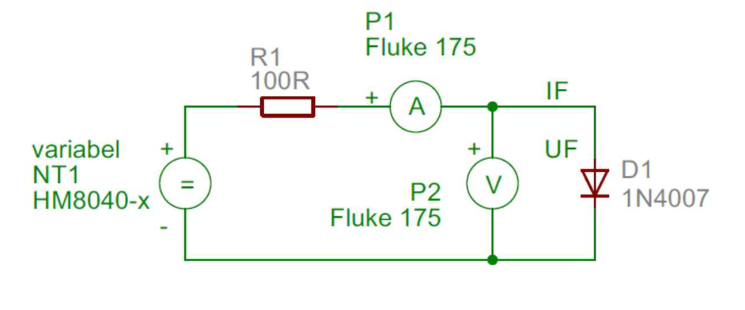
\includegraphics[scale=1.7]{bilder/aufbau_task1a.png}
~
}
\end{figure}


In diesem Fall (Grafik~\ref{fig:aufbau_task1b}) wird stromrichtig gemessen. Der Strom wird allerdings nicht direkt mit Hilfe eines Amperemeters gemessen, sondern durch den Spannungsabfall eines vorgegebenen Widerstandes. Es gilt in diesem Fall für den Strom $I_D$ durch die Diode
\begin{align*}
I_D = \frac{U_\text{IR}}{\text{R2}}
\end{align*}
Da R2 sehr groß ist (1~M$\Omega$), wird ein sehr kleiner Strom (im Bereich von nA) durch die Diode erwartet.

\begin{figure}[H]
\caption{Versuchsaufbau von Aufgabe 1 (b): Gleichrichterdiode in Sperrrichtung}
\label{fig:aufbau_task1b}
{\centering
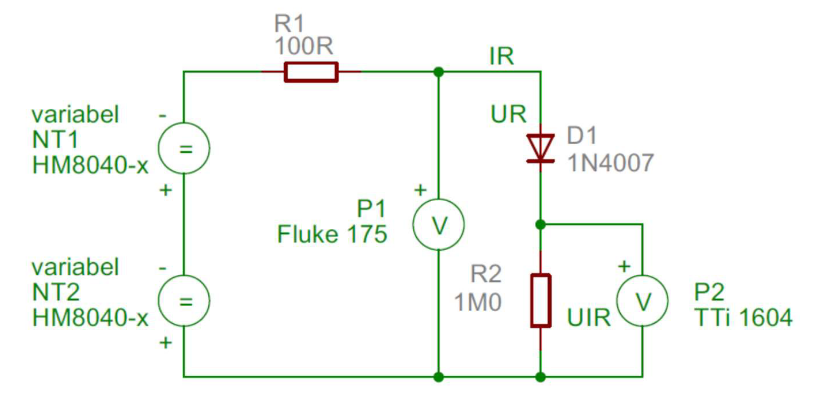
\includegraphics[scale=1.7]{bilder/aufbau_task1b.png}
~
}
\end{figure}

\subsection{Strom-Spannungscharakteristik einer Zenerdiode}

Bei der Zenerdiode wird die Spannung einmal vor und einmal nach dem Widerstand gemessen. Durch die Spannungsdifferenz zwischen vorher und nachher kann aufgrund des Wertes für den Widerstand der Strom bestimmt werden. Damit bekommt man den Strom und die Spannung der Zenerdiode und kann die Kennlinie aufstellen.

\begin{figure}[H]
\caption{Versuchsaufbau von Aufgabe 2}
\label{fig:aufbau_task2}
{\centering
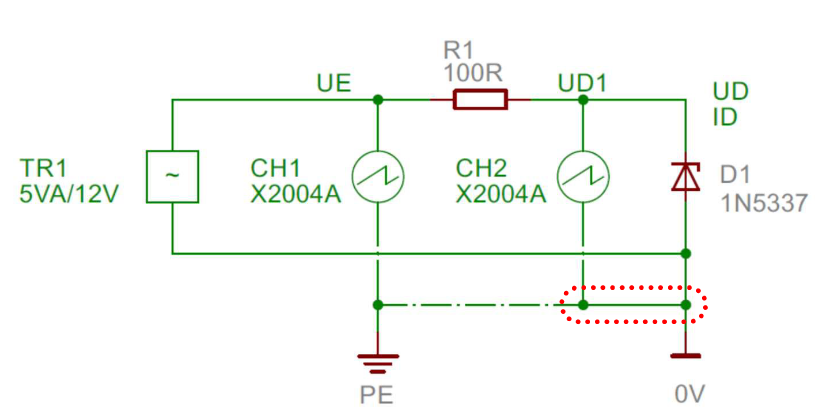
\includegraphics[scale=1.7]{bilder/aufbau_task2.png}
~
}
\end{figure}



\subsection{Einweg- bzw. Gleichrichterschaltung mit unterschiedlichen Glättungskondensatoren und Belastungswiderständen}

Eine Gleichrichterschaltung dient dazu, dass der Verbraucher (R3) nur mit positiver Spannung (Gleichstrom) versorgt wird. Der Transformator TR1 dient als Wechselspannungsquelle. An der Diode D1 wird nur eine positive Spannung durchgelassen. Bei positiver Spannung durch TR1 schaltet die Diode auf Durchlass. Dann wird der Kondensator geladen und R3 mit positiver Spannung versorgt. Bei negativer Spannung durch TR1 sperrt die Diode und der Verbraucher R3 wird wieder mit positiver Spannung des Kondensators versorgt. Der Versuchsaufbau ist in Grafik~\ref{fig:aufbau_task3} zu sehen. Eine zweite Version ohne Messgeräte (Oszilloskop) sieht man zum besseren Verständnis in Grafik~\ref{fig:aufbau_task3_simple}.



Die Spannung an der Diode kann durch Subtraktion der Spannungen aus CH2 und CH4 bestimmt werden.
\begin{align}
U_{\text{D1}} = U_{\text{CH2}} - U_{\text{CH4}}
\end{align}
Der Strom an C1 ist gleich dem Strom an R2, also gilt
\begin{align}
I_{\text{C1}} = \frac{U_{\text{R2}}}{\text{R2}}
\end{align}
Der Strom durch den Verbraucher R3 ist über CH4 zu berechnen
\begin{align}
I_{\text{R3}} = \frac{U_{\text{CH4}}}{\text{R3}}
\end{align}
Der Strom durch die Diode muss auch durch R1 gehen (sieht man in Grafik~\ref{fig:aufbau_task3_simple} besser). Die Spannung über R1 wird bei CH1 gemessen, insgesamt gilt daher
\begin{align}
I_{\text{D1}} = \frac{U_{\text{CH1}}}{\text{R1}}
\end{align}

\begin{figure}[H]
\caption{Versuchsaufbau von Aufgabe 3}
\label{fig:aufbau_task3}
{\centering
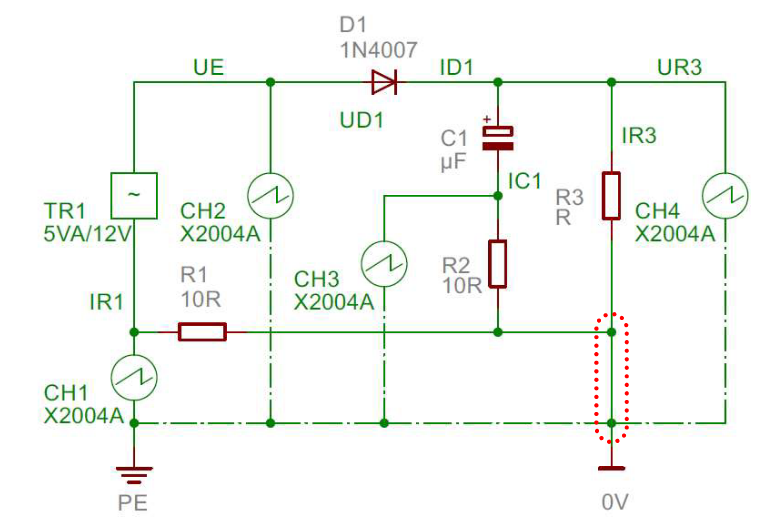
\includegraphics[scale=1.7]{bilder/aufbau_task3.png}
~
}
\end{figure}

\begin{figure}[H]
\caption{Versuchsaufbau von Aufgabe 3, vereinfachte Darstellung ohne Oszilloskop.}
\label{fig:aufbau_task3_simple}
{\centering
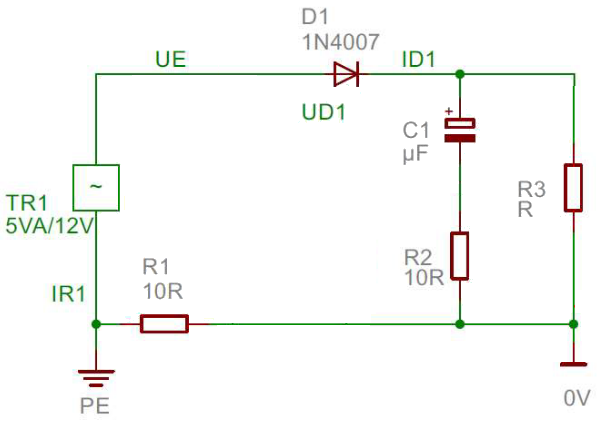
\includegraphics[scale=1.7]{bilder/aufbau_task3_vereinfacht.png}
~
}
\end{figure}



\section{Versuchsdurchführung und Messwerte}

\subsection{Strom-Spannungscharakteristik einer Gleichrichterdiode}

Zuerst wird gemäß Grafik~\ref{fig:aufbau_task1a} in Durchlassrichtung gemessen. Die Messung erfolgt dabei spannungsrichtig. Die Ergebnisse sind in Tabelle~\ref{tab:task1a_daten} zusammengefasst. Beim Aufbau ist auf die korrekte Polung der Geräte zu achten.


\begin{table}[H]
\caption{Messung der Durchlassspannung $U_F$ und des Durchlassstromes $I_F$ an einer Gleichrichterdiode.}
\label{tab:task1a_daten}
\begin{tabular}{r|r}
$U_F$ / V & $I_F$ / mA \\ \hline
0.000 &  0.00   \\
0.110 &  0.01   \\
0.391 &  0.01   \\
0.510 &  0.15   \\
0.595 &  1.02   \\
0.700 & 10.51   \\
0.723 & 14.50   \\
0.735 & 22.16   \\
0.747 & 32.53   \\
0.764 & 50.30   \\
0.780 & 75.60   \\
0.791 & 101.10   \\
0.799 & 125.70   \\
0.806 & 151.80   \\
0.812 & 176.60   \\
0.815 & 192.40
\end{tabular}
\end{table}


Im zweiten Teil wird gemäß Grafik~\ref{fig:aufbau_task1b} gemessen. Diesmal ist die Messung stromrichtig. Zusätzlich werden zwei Netzgeräte in Serie geschalten, um eine höhere Spannung zu erzielen. Der Sperrstrom wird anhand des Spannungsabfalls an einem seriell geschalteten hochomigen Widerstand gemessen. Da bei der Sperrrichtung die Polung vertauscht ist, sind die Spannungen entsprechend negativ.



\begin{table}[H]
\caption{Messung der Sperrspannung \UR und der Sperrstromspannung  \UIR an einer Gleichrichterdiode in Sperrichtung.}
\label{tab:task1b_daten}
\begin{tabular}{r|r}
$U_R$ / V & $U_\text{IR}$ / mV \\ \hline
0   &  0.00 \\
-5  & -0.45 \\
-10 & -0.74 \\
-15 & -1.01 \\
-20 & -1.19 \\
-25 & -1.36 \\
-30 & -1.49 \\
-35 & -1.58 \\
-40 & -1.67
\end{tabular}
\end{table}


\subsection{Strom-Spannungscharakteristik einer Zenerdiode}

Gemäß des Aufbaus in Grafik~\ref{fig:aufbau_task2} folgt durch Messung


\begin{figure}[H]
\caption{Spannungen am Oszilloskop gemäß des Versuchsaufbaus in Grafik~\ref{fig:aufbau_task2}. Auf CH1 liegt die Eingangsspannung des Transformators an, auf CH2 wird die Spannung über die Diode gemessen.}
\label{fig:grafik_task2}
{\centering
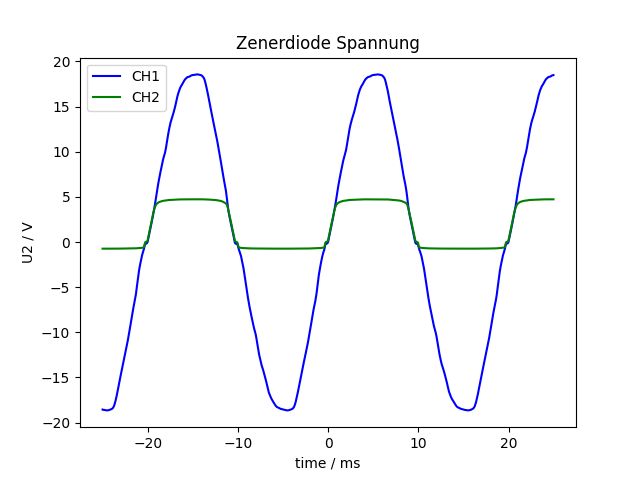
\includegraphics[scale=0.7]{bilder/task2.png}
~
}
\end{figure}

\subsection{Einweg- bzw. Gleichrichterschaltung mit unterschiedlichen Glättungskondensatoren und Belastungswiderständen}

In diesem Fall wird der Versuchsaufbau in Grafik~\ref{fig:aufbau_task3} betrachtet. Bei diesem wird wechselweise der Widerstand R3 (Verbraucher) ausgewechselt. Insgesamt stehen für R3 die Werte $1500~\text{k}\Omega$, $100~\Omega$ und $\infty$ (also keine Verbindung an dieser Stelle) zur Verfügung. Zusätzlich kann der Kondensator C1 des Versuchsaufbaus variieren. Im Versuch stehen die Werte $10~\mu$F und $100~\mu$F zur Verfügung.

Die 3 Werte für den Widerstand R3 und jene 2 Werte für den Kondensator werden kombiniert, sodass insgesamt 6 Messungen durchgeführt werden.


\begin{figure}[H]
\caption{Messung der Einwegschaltung gemäß Versuchsaufbau in Grafik~\ref{fig:aufbau_task3}. $C=10~\mu$F, $R=100~\Omega$}
\label{fig:grafik_task3_10_100}
{\centering
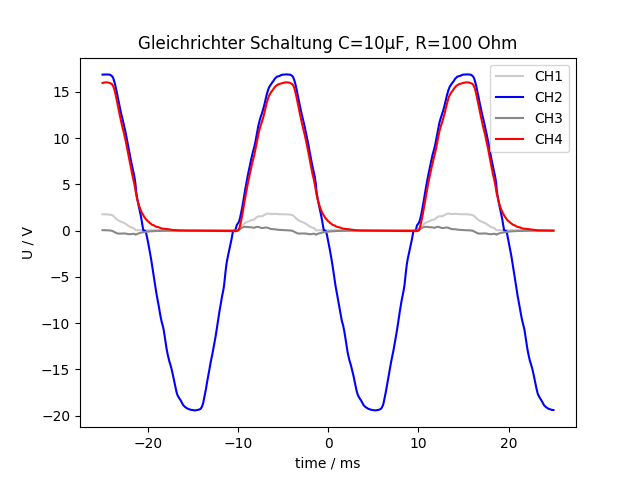
\includegraphics[scale=0.6]{bilder/task3_10mu_R100.png}
~
}
\end{figure}

\begin{figure}[H]
\caption{Messung der Einwegschaltung gemäß Versuchsaufbau in Grafik~\ref{fig:aufbau_task3}. $C=10~\mu$F, $R=1500~\Omega$}
\label{fig:grafik_task3_10_1500}
{\centering
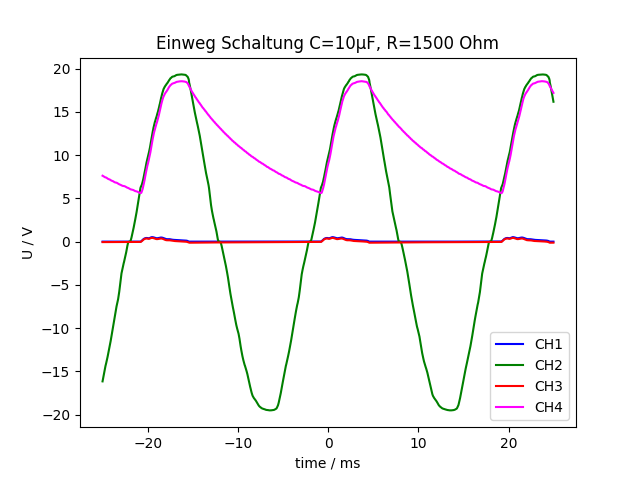
\includegraphics[scale=0.6]{bilder/task3_10mu_R1500.png}
~
}
\end{figure}

\begin{figure}[H]
\caption{Messung der Einwegschaltung gemäß Versuchsaufbau in Grafik~\ref{fig:aufbau_task3}. $C=10~\mu$F, $R=\infty$}
\label{fig:grafik_task3_10_inf}
{\centering
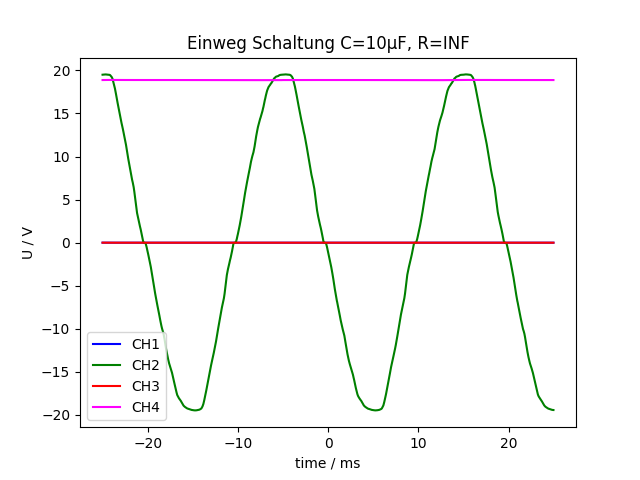
\includegraphics[scale=0.6]{bilder/task3_10mu_Rinf.png}
~
}
\end{figure}





\begin{figure}[H]
\caption{Messung der Einwegschaltung gemäß Versuchsaufbau in Grafik~\ref{fig:aufbau_task3}. $C=100~\mu$F, $R=100~\Omega$}
\label{fig:grafik_task3_100_100}
{\centering
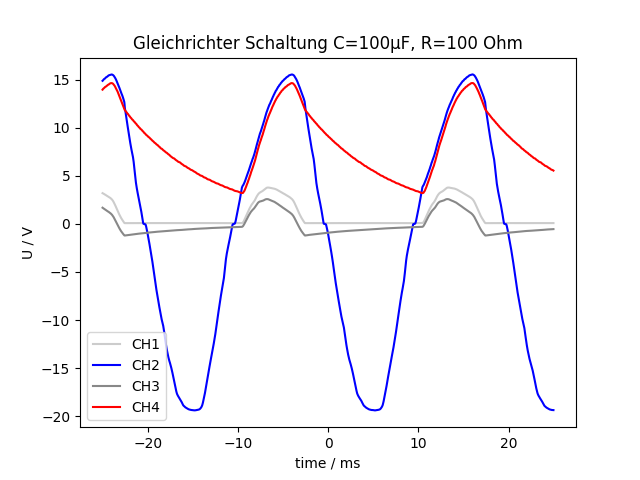
\includegraphics[scale=0.6]{bilder/task3_100mu_R100.png}
~
}
\end{figure}

\begin{figure}[H]
\caption{Messung der Einwegschaltung gemäß Versuchsaufbau in Grafik~\ref{fig:aufbau_task3}. $C=100~\mu$F, $R=1500~\Omega$}
\label{fig:grafik_task3_100_1500}
{\centering
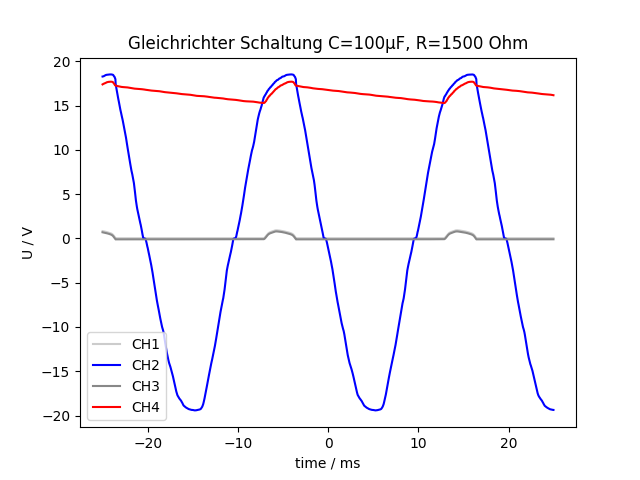
\includegraphics[scale=0.6]{bilder/task3_100mu_R1500.png}
~
}
\end{figure}

\begin{figure}[H]
\caption{Messung der Einwegschaltung gemäß Versuchsaufbau in Grafik~\ref{fig:aufbau_task3}. $C=100~\mu$F, $R=\infty$}
\label{fig:grafik_task3_100_inf}
{\centering
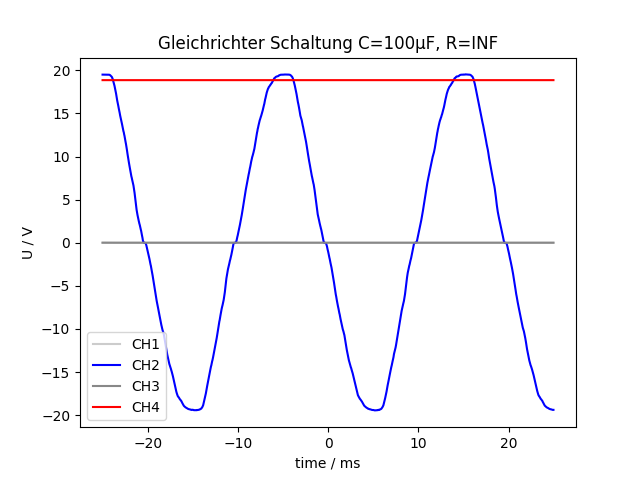
\includegraphics[scale=0.6]{bilder/task3_100mu_Rinf.png}
~
}
\end{figure}




\section{Auswertung}

\subsection{Strom-Spannungscharakteristik einer Gleichrichterdiode}

Aus den gegebenen Werten kann man eine Kennlinie für diese Diode berechnen. Diese ist in Abbildung~\ref{fig:grafik_task1a} dargestellt. 
\begin{figure}[H]
\caption{Durchlassspannung $U_F$ und Durchlassstrom $I_F$ grafisch dargestellt.}
\label{fig:grafik_task1a}
{\centering
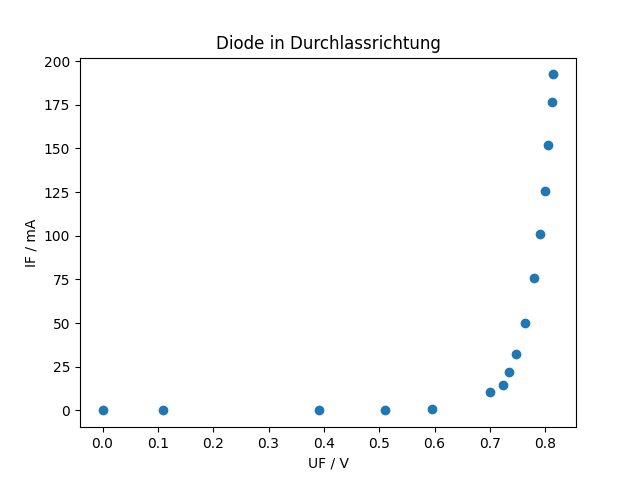
\includegraphics[scale=0.7]{bilder/task1a.png}
~
}
\end{figure}



\begin{table}[H]
\caption{Berechnung des Sperrstromes aus der Sperrstromspannung. Es gilt \UIR $= R\cdot I_R$ mit $R=(1000\pm10)~$k$\Omega$.}
\label{tab:task1b_auswertung}
\begin{tabular}{rr|rr}
$U_R$ / V & $U_\text{IR}$ / mV& $I_R$ / nA & $\Delta I_R$ / nA \\ \hline
0   &  0.00 & 0.00 \\
-5  & -0.45 & -0.45 \\
-10 & -0.74 & -0.74 \\
-15 & -1.01 & -1.01 \\
-20 & -1.19 & -1.19 \\
-25 & -1.36 & -1.36 \\
-30 & -1.49 & -1.49 \\
-35 & -1.58 & -1.58 \\
-40 & -1.67 & -1.67
\end{tabular}
\end{table}


\begin{figure}[H]
\caption{Sperrspannung $U_R$ und Sperrstrom $I_R$ grafisch dargestellt.}
\label{fig:grafik_task1b}
{\centering
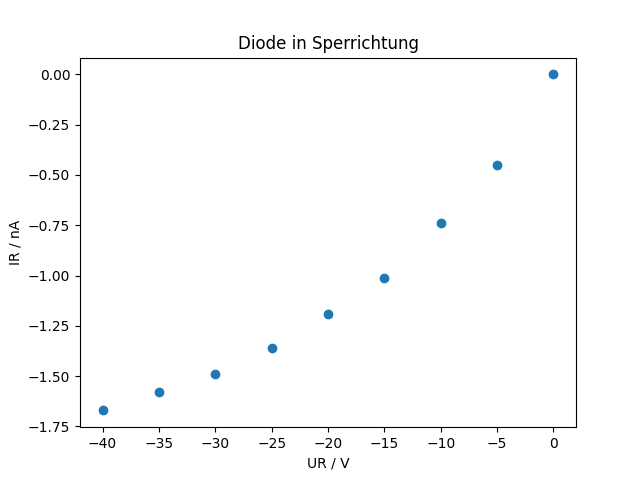
\includegraphics[scale=0.7]{bilder/task1b.png}
~
}
\end{figure}

\subsection{Strom-Spannungscharakteristik einer Zenerdiode}

In diesem Versuch ist der Strom durch die Diode zu berechnen. Gemäß des Versuchsaufbaus in Grafik~\ref{fig:grafik_task2} und den Informationen im Moodle (\cite{moodle}), gilt
\begin{align*}
I_D = \frac{U_2-U_1}{R_1}
\end{align*}
Der zeitliche Verlauf des Stromes ist in Grafik~\ref{fig:task2_auswertung1} veranschaulicht.

\begin{figure}[H]
\caption{Stromverlauf durch die Zenerdiode.}
\label{fig:task2_auswertung1}
{\centering
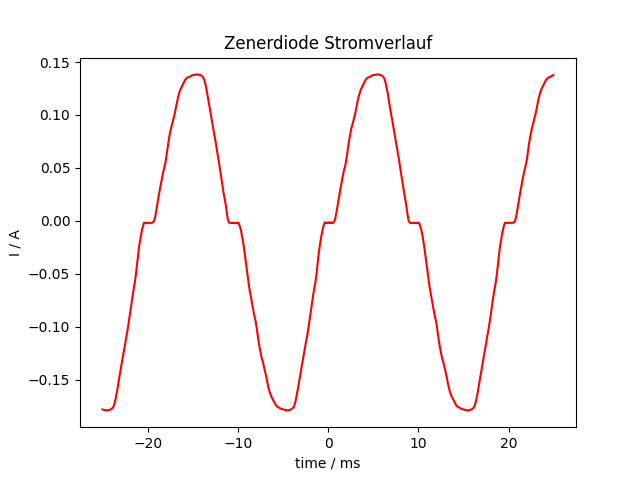
\includegraphics[scale=0.6]{bilder/task2_I.png}
~
}
\end{figure}




\begin{figure}[H]
\caption{Kennlinie der Zenerdiode.}
\label{fig:task2_auswertung2}
{\centering
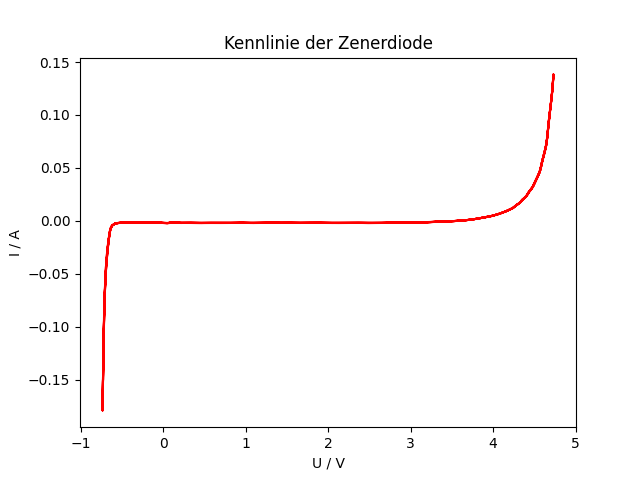
\includegraphics[scale=0.6]{bilder/task2_IU.png}
~
}
\end{figure}



\subsection{Einweg- bzw. Gleichrichterschaltung mit unterschiedlichen Glättungskondensatoren und Belastungswiderständen}



\section{Diskussion}

\subsection{Strom-Spannungscharakteristik einer Gleichrichterdiode}

Die Strom-Spannungscharakteristik wurde in den Grafiken~\ref{fig:grafik_task1a} und \ref{fig:grafik_task1b} dargestellt. Bei der Durchlassrichtung ist eine Erhöhung des Stromes zwischen 0.7~V und 0.8~V zu erkennen. Gemäß des Datenblattes von IN4007 Dioden (\cite{conrad_diode1}), sieht man hier eine Übereinstimmung. Das Verhalten ist damit konform mit den Erwartungen. Über die Sperrrichtung lässt das Datenblatt nichts aussagen, da im Datenblatt der Sperrstrom als $<5~\mu$A (bzw. $<50~\mu$A bei 100$^\circ$C) charakteristiert ist. Spannungen im Bereich von Nanoampere sind daher zu vernachlässigen. Um den Strom zu erhöhen, müsste eine Durchbruchspannung angelegt werden, die deutlich größer ist. Dadurch würde die Diode zerstört werden.



\subsection{Strom-Spannungscharakteristik einer Zenerdiode}



\section{Zusammenfassung}




\begin{thebibliography}{9}
\bibitem{moodle} Moodle-Unterlagen zum Versuch, bereitgestellt von der Karl-Franzens-Universität Graz.
\bibitem{halbleiter} \url{https://www.chemie.de/lexikon/Halbleiter.html}, 22.11.2020 23:25.
\bibitem{cosmos} \url{https://physik.cosmos-indirekt.de/Physik-Schule/Bändermodell}, 22.11.2020 23:28.
\bibitem{greenlane} \url{https://www.greelane.com/wissenschaft-technologie-mathematik/wissenschaft/examples-of-electrical-conductors-and-insulators-608315/}, 22.11.2020 23:29.
\bibitem{lernhelfer} \url{https://www.lernhelfer.de/schuelerlexikon/physik/artikel/halbleiter}, 22.11.2020 23:32.
\bibitem{leifiphysik} \url{https://www.leifiphysik.de/elektronik/einfuehrung-die-elektronik/grundwissen/dotierte-halbleiter}, 22.11.2020 23:40.
\bibitem{leifiphysik2} \url{https://www.leifiphysik.de/elektronik/halbleiterdiode/grundwissen/p-n-uebergang-halbleiterdiode}, 24.11.2020 00:08.
\bibitem{kompendium} \url{https://www.elektronik-kompendium.de/sites/grd/0112072.htm}, 24.11.2020 00:09.
\bibitem{conrad_diode1} \url{https://asset.conrad.com/media10/add/160267/c1/-/gl/000162272DS01/datenblatt-162272-diotec-si-gleichrichterdiode-1n4007-do-204al-1000-v-1-a.pdf},28.11.2020, 09:22.
\bibitem{conrad_diode2} \url{https://asset.conrad.com/media10/add/160267/c1/-/en/000168265DS01/datenblatt-168265-on-semiconductor-z-diode-1n5337brlg-gehaeuseart-halbleiter-axial-zener-spannung-47-v-leistung-max-ptot-5-w.pdf}, 28.11.2020, 09:35.
\end{thebibliography}


%\newpage 
%\appendix
%\section{Python Skript}



\definecolor{commentgreen}{RGB}{2,112,10}
\definecolor{eminence}{RGB}{108,48,130}
\definecolor{weborange}{RGB}{255,165,0}
\definecolor{frenchplum}{RGB}{129,20,83}

\lstdefinelanguage{python}{
    morekeywords={def, for, range, abs, return},
    otherkeywords={<-,->, |>, \%\{, \}, \{, \, (, )},
    sensitive=true,
    morecomment=[l]{\#},
    morecomment=[n]{/*}{*/},
    morecomment=[s][\color{purple}]{:}{\ },
    morestring=[s][\color{orange}]"",
    commentstyle=\color{commentgreen},
    keywordstyle=\color{eminence},
    stringstyle=\color{red},
	basicstyle=\ttfamily,
	breaklines,
	showstringspaces=false,
	frame=tb
}
\lstset{
extendedchars=\true,
inputencoding=utf8
}

%\lstinputlisting[language=Python,captionpos=b, label=lst:test,caption={Python Skript}]{plot.py}

%\lstinputlisting[language=Python,captionpos=b, label=lst:test,caption={Bessel Auswertung}]{generate_numbers_bessel.py}


%\lstinputlisting[language=Python,captionpos=b, label=lst:test,caption={Zerstreuungslinse Auswertung}]{generate_numbers_zerstreuungslinse.py}


\end{document}
